% =====================================================================================================
% Kapitel 6: Versetzen des IO-Link-Masters                                      Zielumfang: ca. 4 Seiten
% Sicherheitshinweis: Umbau nur freigeschaltet und gegen Wiedereinschalten gesichert.
% =====================================================================================================

\section{Versetzen des IO-Link-Masters}

\subsection{Analyse der Ausgangssituation}
% INHALT:  - aktuelle Position des AL1100 auf der Schleppkette (Foto), Masse von Master + Leitungen
%            (gewogen oder Datenblatt), Auswirkungen auf Kette und Antrieb
%          - angeschlossene Devices: Port 1 DTI515, Port 2 OY5100; PROFINET- und Versorgungsleitung
% QUELLEN: Datenblatt AL1100, Vorgänger-T3100 (Abb. Portbelegung)
% UMFANG:  ca. 1 Seite
%
% MATERIAL AUS DEM INTERVIEW (05.11.2026) – Umbau ist bereits erfolgt, Fotos folgen:
%   Mechanik Regalbediengerät:
%   - untere Achse links/rechts (horizontal), mit Schleppkette
%   - darauf zweite Achse hoch/runter (vertikal); an ihr ist der Druckluftzylinder befestigt
%     (fährt ein/aus, legt Klotz/Palette ins Fach)
%   - RFID-Lesekopf vorne am Zylinder (erkennt, welches Material gerade bewegt wird)
%   Alter Zustand:
%   - IO-Link-Master saß auf der verfahrbaren Einheit (Horizontalachse)
%   - dadurch liefen alle Leitungen des Masters (Versorgung, Netzwerk, Lichtgitter, RFID) durch die
%     Schleppkette; später kamen noch die Lichtgitter-Leitungen dazu
%   - Folge: zu viele Kabel und zu viel Gewicht → Modell konnte nicht mehr sauber verfahren,
%     obwohl eigentlich nur eine kleine Leitung (RFID) mitfahren muss
%   Neuer Zustand:
%   - Master fest montiert nahe den Lichtgittern (genaue Position: TODO, Foto)
%   - nur noch die kleine RFID-Leitung läuft durch die Schleppkette hoch zum Zylinder
%   Leitungen am Master:
%   - 1 Leitung mit Y-Aufteilung auf 2 → Lichtgitter (Sender/Empfänger)
%   - 1 Leitung Versorgungsspannung
%   - 1 Leitung Netzwerk (PROFINET)
%   - 1 Leitung RFID-Lesekopf
%   (Port-Zuordnung prüfen)
%   - Versorgung und Netzwerk sind getrennte Leitungen (kein PoE)
%   Ergebnis:
%   - Umbau abgeschlossen, Anlage funktioniert nach dem Umsetzen weiterhin vollständig
%   - im TIA-Projekt war keine Änderung nötig (Gerätename/Ports unverändert)
%   - Testablauf und Datum für 6.4 noch festhalten (TODO)

% --- Abbildungen (Auswahl aus Fotos vom 05.11.2026; im Text mit \ref{} referenzieren) ---
\begin{figure}[H]
  \centering
  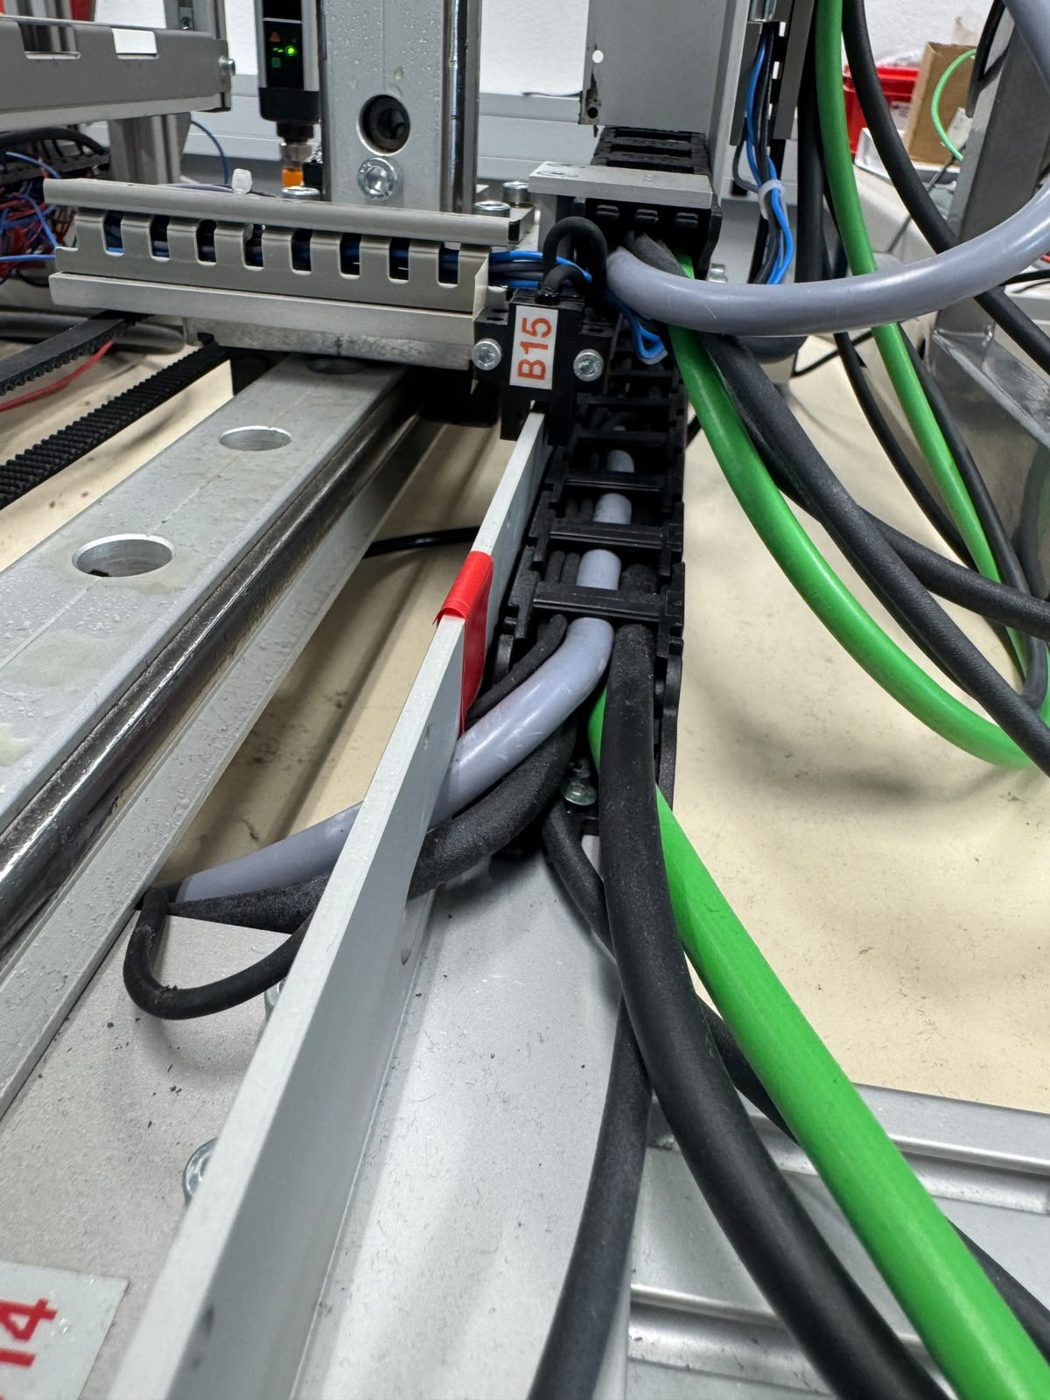
\includegraphics[height=0.4\textheight]{images/schleppkette_leitungen.jpg}
  \caption{Leitungen in der Schleppkette der Horizontalachse \quelle{(eigene Aufnahme, 11/2026)}}
  \label{fig:schleppkette}
\end{figure}

\begin{figure}[H]
  \centering
  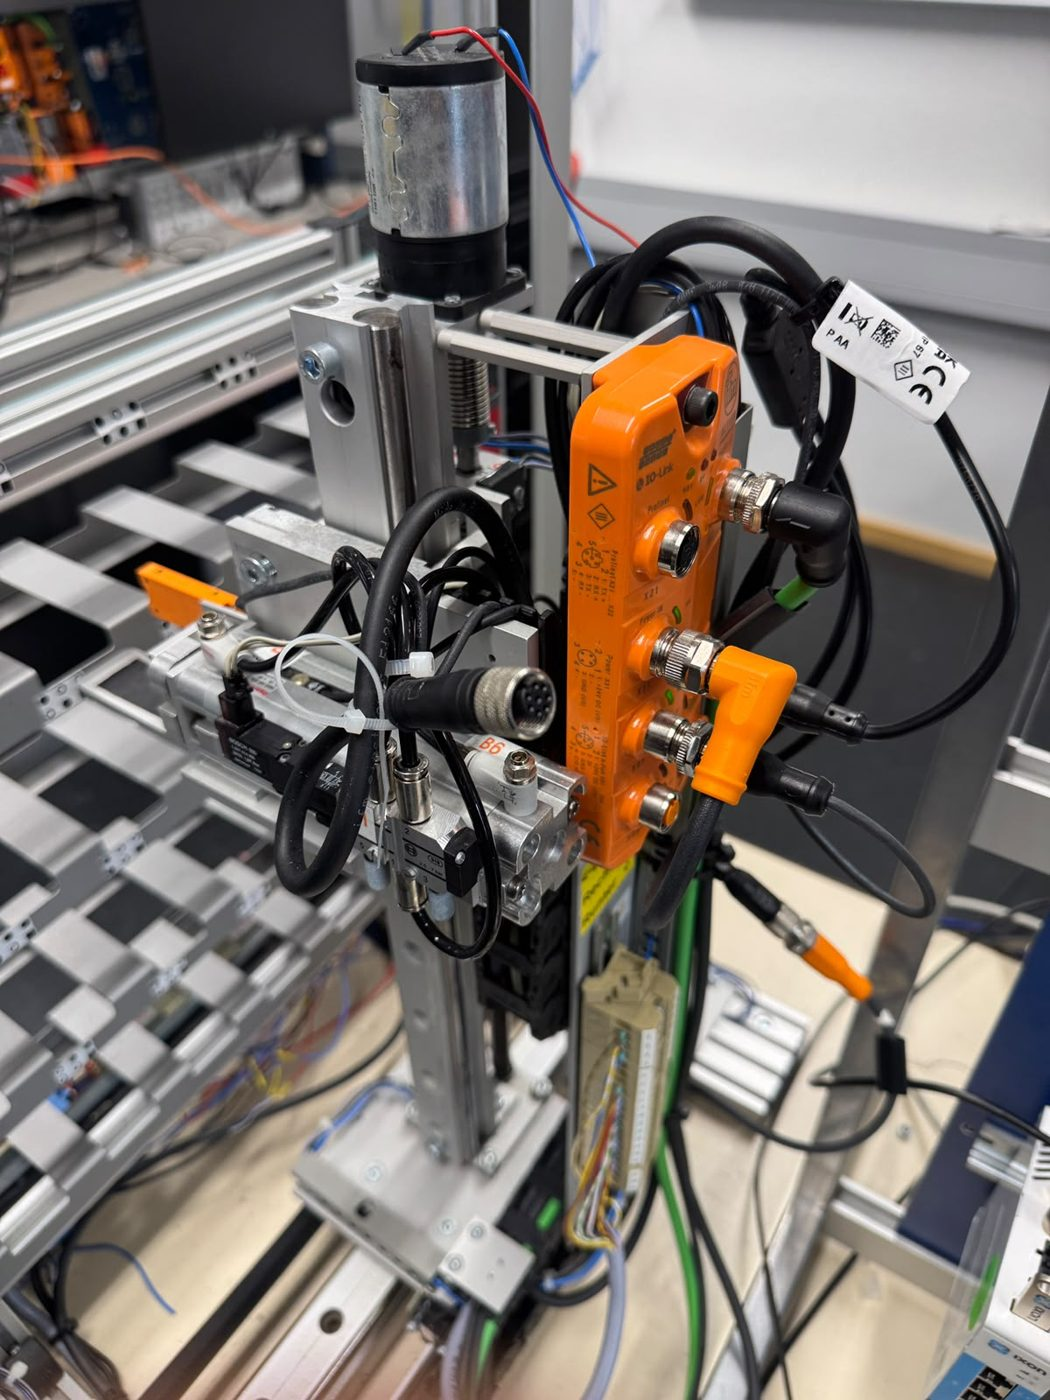
\includegraphics[height=0.4\textheight]{images/iolink_master_position.jpg}
  \caption{Montageposition des IO-Link-Masters AL1100 (TODO: vorher/nachher zuordnen) \quelle{(eigene Aufnahme, 11/2026)}}
  \label{fig:al1100_position}
\end{figure}

\begin{figure}[H]
  \centering
  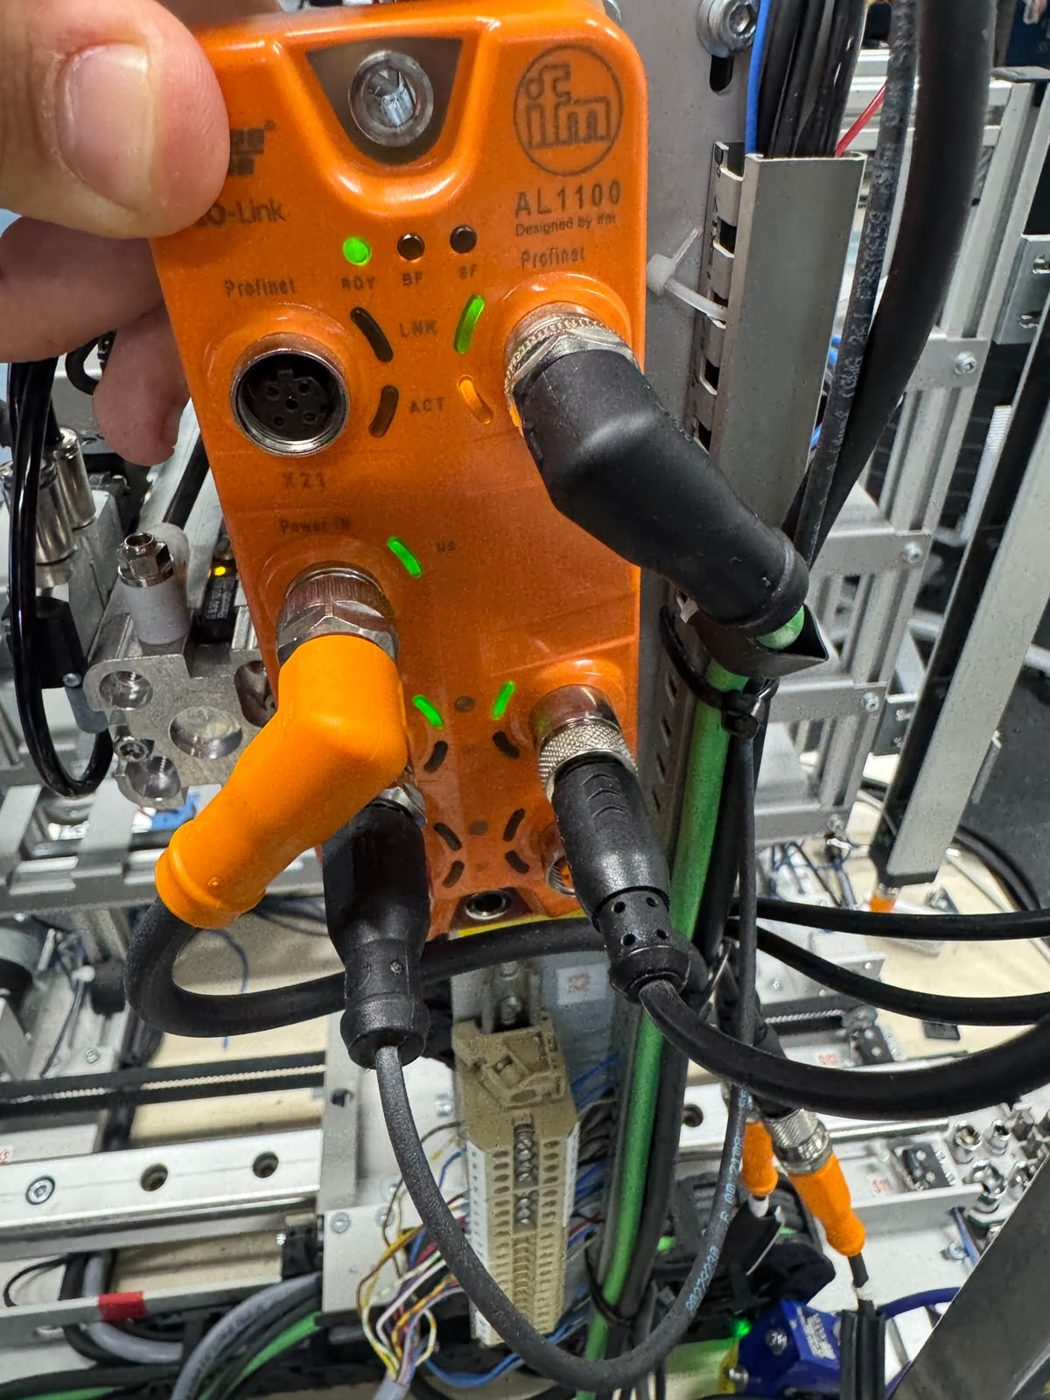
\includegraphics[height=0.4\textheight]{images/iolink_master_al1100.jpg}
  \caption{IO-Link-Master ifm AL1100 mit belegten Ports \quelle{(eigene Aufnahme, 11/2026)}}
  \label{fig:al1100_detail}
\end{figure}

\begin{figure}[H]
  \centering
  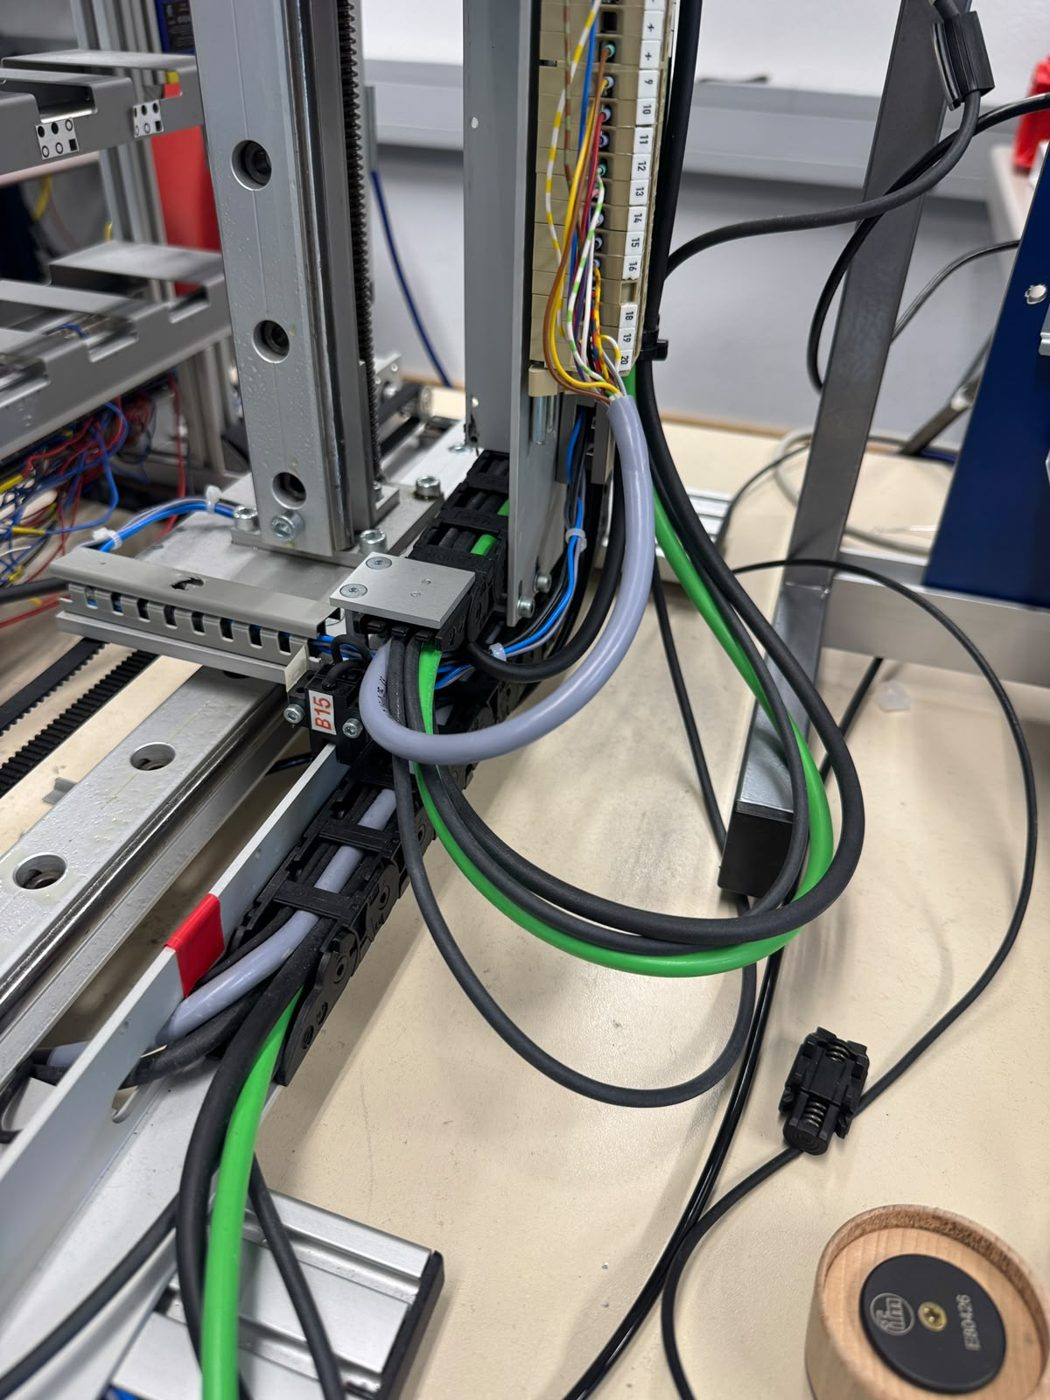
\includegraphics[height=0.4\textheight]{images/iolink_y_verteiler_lichtgitter.jpg}
  \caption{Y-Verteiler für Sender und Empfänger des Lichtgitters \quelle{(eigene Aufnahme, 11/2026)}}
  \label{fig:y_verteiler}
\end{figure}

\begin{figure}[H]
  \centering
  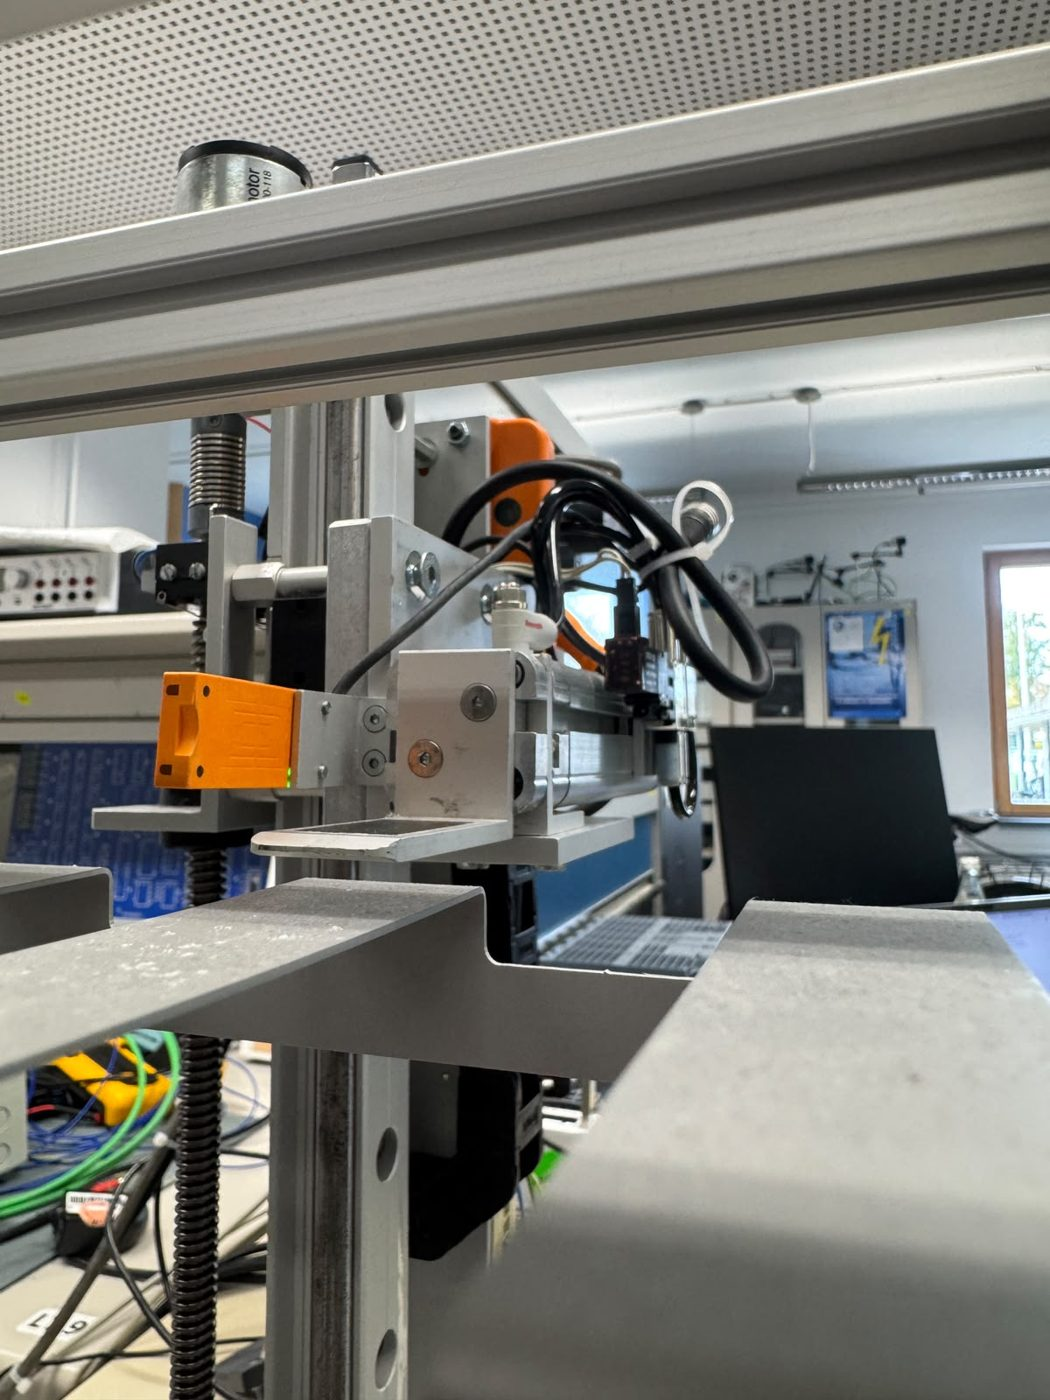
\includegraphics[height=0.4\textheight]{images/rfid_lesekopf_zylinder.jpg}
  \caption{RFID-Lesekopf an der Vorderseite des Zylinders \quelle{(eigene Aufnahme, 11/2026)}}
  \label{fig:rfid}
\end{figure}

\subsection{Auswahl des neuen Montageorts}
% INHALT:  - Kriterien: feste Position, Leitungslängen zu den Devices (Grenze IO-Link → Quelle),
%            Zugänglichkeit, Kabelführung durch die Kette
%          - ggf. Variantenvergleich (Tabelle), Entscheidung mit Begründung
% UMFANG:  ca. 1 Seite

\subsection{Umbau}
% INHALT:  - Vorgehen, neue Leitungsführung (Skizze), Fotos nachher
%          - PROFINET-Gerätename und Portbelegung unverändert → keine Änderung im TIA-Projekt nötig
%            (prüfen und so dokumentieren)
% UMFANG:  ca. 1 Seite

\subsection{Inbetriebnahme und Test}
% INHALT:  - Prüfprotokoll: Master online, Devices erkannt, Prozesswerte RFID/Lichtgitter plausibel,
%            Fahrt über gesamten Verfahrweg ohne Leitungszug
% UMFANG:  ca. 0,5 Seiten

\subsection{Fazit}
% INHALT:  Ergebnis bezogen auf Ziel 3, Überleitung zu Kapitel 7
